\subtop{Hochdimensionale Daten}{-1.45}
\subsection{geometrisch-transformierte Displays}
\begin{itemize}
	\item Projektion von $n$ Datendimensionen auf $k$ Displaydimensionen
	\item jeder Record in der Projektion ist ein visuelles Zeichen (Mark)
	\item es gibt verschiedene Projektionstechniken (z.B. PCA, MDS)
	\item Beispiele:
		\begin{description}
			\item[Scatterplot-Matrizen]
			\item[Landscapes]
			\item[Force-Based Methoden / RaddViz] \ \\\vspace*{-\baselineskip}
				\begin{itemize}
					\item schwierig für zu viele Dimensionen
					\item Beispiel: MDS
					\item möglicherweise Infos in Visualisierung aber nicht in den Daten
				\end{itemize}
			\item[Tabular Displays] \ \\\vspace*{-\baselineskip}
				\begin{itemize}
					\item Farbe, Größe/Länge als Datenkodierung
					\item Darstellung in Tabelle
				\end{itemize}
			\item[Parallel Coordinates]
			\item[Dimensionales Stacking]\ \\\vspace*{-\baselineskip}
				\begin{itemize}
					\item $n$-dimensionale Daten werden auf $2$-dimensionales Bild gemappt
					\item starten mit $2n+1$ dimensionalen Daten
					\item feste Größe für jede Dimension festlegen
					\item eine Dimension: abhängige Variable
					\item alle weiteren Dimensionen: unabhängige Variablen
				\end{itemize}
				\usetikzlibrary{positioning}
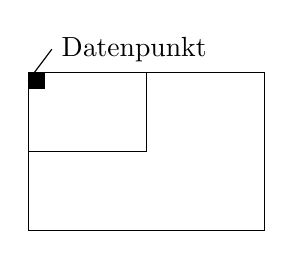
\begin{tikzpicture}[]

\draw (0,0) rectangle (3,2);
\draw (0,2) rectangle (1.5,1);
\draw[fill] (0,2) rectangle (0.2,1.8);

\draw (0,1.9) -- (0.3,2.3);
\node[anchor=west] at (0.3,2.3) {Datenpunkt};
\end{tikzpicture}
		\end{description}
\end{itemize}
%------------------------------------------%
\subsection{Dense-Pixel Displays}
\begin{itemize}
	\item jeder gefärbte Pixel repräsentiert einen Wert
	\item alle Attributwerte in seperaten Unterfenstern
	\item Anordnung der Pixel:
		\begin{itemize}
			\item Peano-Hilbert
			\item Morton (Z-Curve)
			\item rekursive Pattern Technik
		\end{itemize}
	\item Form der Unterfenster: Pixel des selben Datenpunktes sollen nah bei einander sein
	\item Anordnung der Dimensionen: ähnliche Dimensionen nah beieinander
\end{itemize}
\topbreak
\vspace*{-1.5\baselineskip}
%------------------------------------------%
\subsection{Pixel Bar Chart}
	\begin{itemize}
		\item Probleme:
			\begin{itemize}
				\item bar charts zeigen nur einen Teil der Daten
				\item Scatterplots haben viel overlap
				\item pixel-displays brauchen Pixel-Zusammenhang
			\end{itemize}
		\item Definition:
			\begin{itemize}
				\item $\left<D_x,D_y, O_x,O_y,C\right>$
				\item $D_x,D_y$ sind Teilungsattribute für $x$- und $y$-Achse
				\item $O_x,O_y$ sind Reihenfolgeattribute für $x$- und $y$-Achse
				\item $C$ ist (sind) Farbattribut(e)
			\end{itemize}
		\item Formalisierung des Pixel-Positionierungsproblems:
			\begin{description}
				\item[Dense-Display-Constraint] Display ist vollständig mit Pixeln gefüllt
				\item[No-Overlap-Constraint] keine doppelte Belegung einer Position (jedes Pixel hat seine eigene Position)
				\item[Locality-Constraint] ähnliche Pixel liegen nah bei einander
				\item[Ordering-Constraint] Reihenfolge auf $x$- und $y$-Achse wird erzwungen
			\end{description}
		\item Heuristik für Pixel-Positionierung:
			\begin{enumerate}
				\item Quantile für $x$- und $y$-Achse bestimmen
				\item erstes Pixel unten links platzieren
				\item Pixel links und unten positionieren
				\item restliche Pixel positionieren
			\end{enumerate}
	\end{itemize}
%------------------------------------------%
\subsection{Color Icons}
Array von Farbfeldern, die Attributwerte darstellen

%------------------------------------------%
\subsection{Vergleich der Techniken}
\begin{description}
	\item[Kriterien] \ \\\vspace*{-\baselineskip}
		\begin{itemize}
			\item Aufgabencharakteristiken (Clustering, multi-mannigfaltige Hot Spots, $\dots$)
			\item Datencharakteristiken (Anzahl mannigfaltiger Datenitems, kategorische Daten, $\dots$)
			\item Visualisierungscharakteristiken (visuelle Overlaps, Lernkurven, $\dots$)
		\end{itemize}
	\item[Vergleich] \ \\\vspace*{-\baselineskip}
		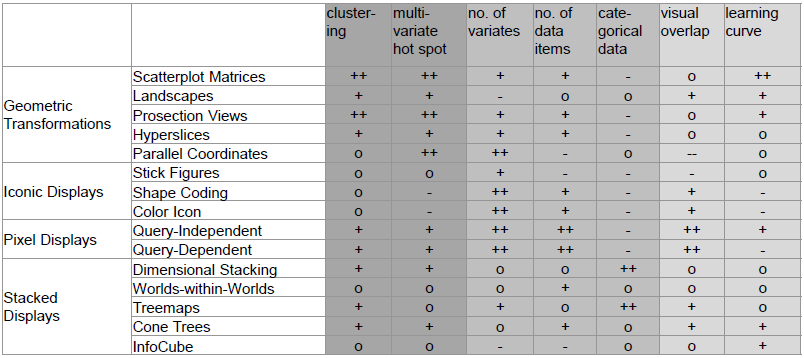
\includegraphics[width=0.98\textwidth]{Pics/03-01-Vergleich.png}
\end{description}
\topbreak
\vspace*{-1.5\baselineskip}
\begin{description}
	\item[Hybrid-Ansätze] \ \\\vspace*{-\baselineskip}
		\begin{itemize}
			\item möglicherweise zusätzliche Informationen darstellbar
			\item virtuell werden alle Visualisierungstechniken mit Dynamiken und Interaktionen kombiniert
		\end{itemize}
	\item[Mehrfach-Ansichten] \ \\\vspace*{-\baselineskip}
		\begin{itemize}
			\item wann?
				\begin{description}
					\item[Rule of Diversity] Vielfalt in Attributen, Modellen, Benutzerprofilen, Abstraktionsleveln, Genres
					\item[Rule of Complementary] unterschiedliche Sichten zeigen Korrelationen oder Ungleichheiten
					\item[Rule of Decomposition] komplexe Daten in mehreren Sichten aufteilen für besseren Einblick in unterschiedliche Attribute
					\item[Rule of Parsimony (Sparsamkeit)] minimale Anzahl an mehreren Sichten
				\end{description}
			\item wie?
				\begin{description}
					\item[Rule of Space/Time Resource Optimization] Nutzen der Darstellung muss mit dem Zeitaufwand zur Berechnung ausbalanciert sein
					\item[Rule of Self-Evidence] Verknüpfung der einzelnen Ansichten
					\item[Rule of Consistency] Interface und Sichten müssen konsistent sein
					\item[Rule of Attention Management] Wahrnehmungstechniken verwenden, um Fokus des Benutzers richtig zu setzen
				\end{description}
		\end{itemize}
\end{description}